\section{Emergence of Symmetry from Closure Geometry}
\label{sec:symmetry}

\subsection{Reversing the Perspective}

In conventional formulations of particle physics,
gauge symmetries such as $\mathrm{SU}(3)$, $\mathrm{SU}(2)$, and $\mathrm{U}(1)$
are introduced as fundamental principles.
Within the present framework, the perspective is reversed.
Since particles are interpreted as stable configurations of triangular closure,
the relevant question becomes:
\begin{equation}
  \boxed{\text{What transformations preserve closure structure?}}
\end{equation}
Symmetry is not assumed a priori; it is identified through invariance of structure.

\subsection{Definition of Symmetry}

A symmetry is defined operationally as:
\begin{equation}
  \boxed{\text{A transformation that preserves closure conditions.}}
\end{equation}
The closure condition consists of vector balance, internal consistency,
and non-degeneracy (when applicable).
Admissible transformations must leave invariant
$\vec{e}_i + \vec{e}_j + \vec{e}_k \approx 0$
and the associated relational structure.

\subsection{Non-Degenerate Triangle and \texorpdfstring{$\mathrm{SU}(3)$}{SU(3)}}

A non-degenerate triangular closure has three internal components
subject to one constraint:
\begin{equation}
  \vec{e}_1 + \vec{e}_2 + \vec{e}_3 = 0.
\end{equation}
Transformations acting on these internal components must preserve
the closure condition and inner products (interaction structure).
This leads naturally to unitary transformations:
\begin{equation}
  \psi \mapsto U\psi, \qquad U^\dagger U = \mathbf{1}.
\end{equation}
Fixing the overall scale ($\det U = 1$) yields:
\begin{equation}
  \boxed{
    \mathrm{SU}(3) \;\text{can be identified as a minimal transformation group
    consistent with the invariance of non-degenerate triangular closure.}
  }
\end{equation}

\subsection{Degenerate Triangle and \texorpdfstring{$\mathrm{SU}(2)$}{SU(2)}}

When the triangle degenerates, one directional degree of freedom is effectively lost.
The structure reduces to two distinguishable internal states.
Transformations preserving this reduced closure structure
act on a two-dimensional internal space:
\begin{equation}
  \begin{pmatrix}|L\rangle\\|R\rangle\end{pmatrix}
  \;\longrightarrow\;
  U\begin{pmatrix}|L\rangle\\|R\rangle\end{pmatrix},
  \qquad U \in \mathrm{SU}(2).
\end{equation}
\begin{equation}
  \boxed{
    \mathrm{SU}(2) \;\text{is associated with the internal degrees of freedom
    of degenerate triangular closure.}
  }
\end{equation}

\subsection{Global Phase and \texorpdfstring{$\mathrm{U}(1)$}{U(1)}}

There exists a transformation that uniformly rescales all internal vectors
by a phase:
\begin{equation}
  \vec{e}_i \;\rightarrow\; e^{i\theta}\vec{e}_i.
\end{equation}
This transformation preserves the closure condition and does not alter
relative structure; it represents a redundancy rather than a physical change.
\begin{equation}
  \boxed{
    \mathrm{U}(1) \;\text{is a global phase symmetry that leaves
    closure structure invariant.}
  }
\end{equation}

\subsection{Structural Correspondence}

The correspondence between closure structure and transformation groups
is summarized in Table~\ref{tab:symmetry} and Fig.~\ref{fig:symmetry}.

\begin{table}[h]
  \centering
  \begin{tabular}{ll}
    \toprule
    Closure structure & Associated symmetry \\
    \midrule
    Non-degenerate triangle & $\mathrm{SU}(3)$ \\
    Degenerate triangle     & $\mathrm{SU}(2)$ \\
    Global phase redundancy & $\mathrm{U}(1)$  \\
    \bottomrule
  \end{tabular}
  \caption{Correspondence between closure regimes and symmetry groups.}
  \label{tab:symmetry}
\end{table}

\begin{equation}
  \boxed{
    \mathrm{SU}(3)\times\mathrm{SU}(2)\times\mathrm{U}(1)
    \;\text{emerges as the symmetry structure of closure geometry.}
  }
\end{equation}

\begin{figure}[h]
  \centering
  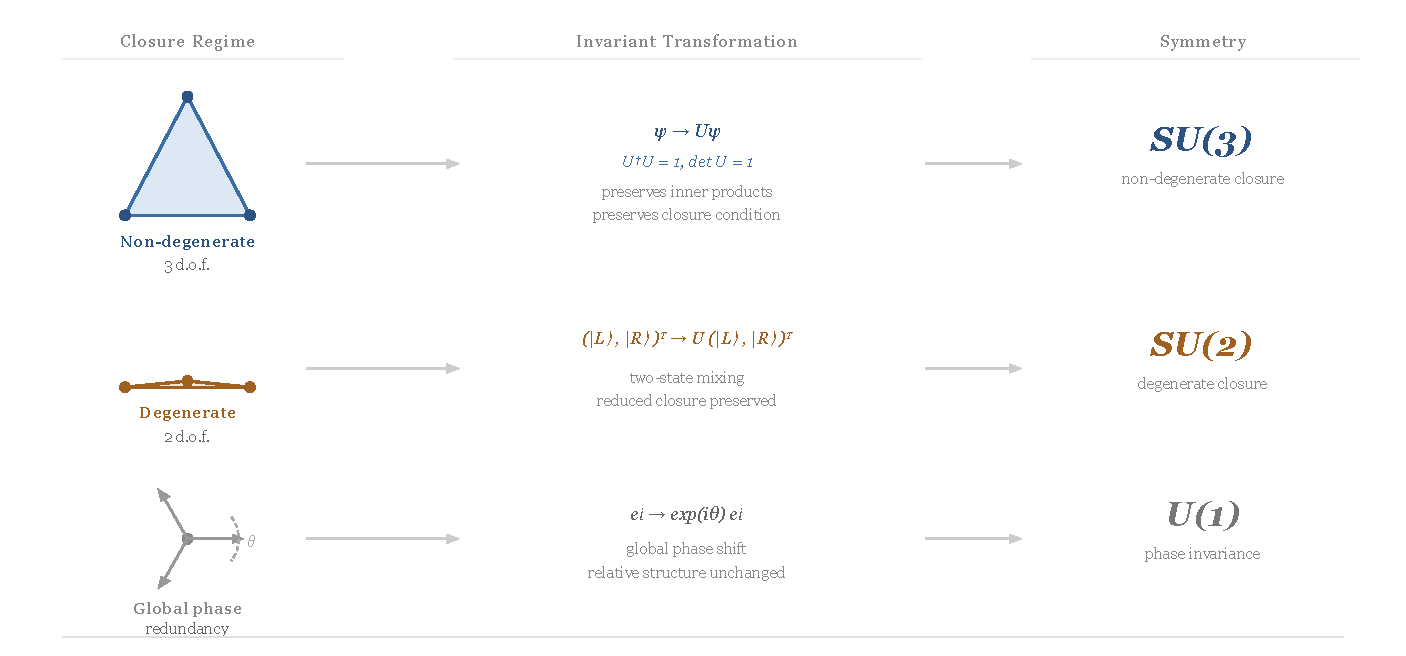
\includegraphics[width=\textwidth]{figures/VED_Vol2_Figure2.pdf}
  \caption{
    Symmetry structure as invariance of closure geometry.
    Distinct closure regimes admit distinct classes of transformations
    that preserve their internal structure.
    Non-degenerate triangular closure is associated with $\mathrm{SU}(3)$,
    degenerate closure with $\mathrm{SU}(2)$,
    and global phase redundancy with $\mathrm{U}(1)$.
    Symmetry is interpreted not as a starting assumption,
    but as the class of admissible transformations preserving closure.
  }
  \label{fig:symmetry}
\end{figure}

\subsection{The Inversion}

The conventional logical order is:
$\text{symmetry} \;\rightarrow\; \text{particle}.$
The present framework reverses this:
\begin{equation}
  \boxed{\text{closure structure} \;\rightarrow\; \text{allowed transformations (symmetry).}}
\end{equation}
Symmetry is therefore not a starting assumption,
but a reflection of structural invariance.
